\documentclass{article}

\usepackage[a4paper,top=1cm,bottom=1cm,left=1cm,right=1cm]{geometry}
\pagenumbering{gobble}
\setlength{\parindent}{0pt}
\usepackage{tgadventor}
\renewcommand*\familydefault{\sfdefault}
\usepackage[T1]{fontenc}
\usepackage{ragged2e}
\usepackage{graphicx} 
\usepackage{float}
\usepackage{wrapfig}
\usepackage{fontawesome5}
\usepackage{tikz}
\usepackage{tikzsymbols}
\usetikzlibrary{positioning}
\usepackage{pgffor}
\usepackage{caption}
\usepackage{multirow}
\usepackage{multicol}

\title{\Huge Escursione: Slittata a malga Gurndin}
\date{}
\author{}

\begin{document}
\newcommand{\stanchezza}[2]{
\begin{tikzpicture}
    \node () at (-2,0) {LIVELLO DI STANCHEZZA};
    \foreach \i in {1,...,#1}{
    \node (\i) at (\i,0) {\Large\faBatteryFull}; }
    \ifnum #2>#1
        \foreach \i in {#1+1,...,#2}{
        \node (\i) at (\i,0) {\Large\faBatteryEmpty}; 
        }
    \fi
\end{tikzpicture}    
}

\newcommand{\esperienza}[2]{
\begin{tikzpicture}
    \node () at (-2,0) {VALUTAZIONE ESPERIENZA};
    \foreach \i in {1,...,#1}{
    \node (\i) at (\i,0) {\Large\faGrinStars}; }

    \ifnum #2>#1
        \foreach \i in {#1+1,...,#2}{
        \node (\i) at (\i,0) {\Large\faGrinStars[regular]};
        }
    \fi
        
\end{tikzpicture}    
}
\begin{tikzpicture}[main/.style = {draw, rectangle, rounded corners=0.1cm,minimum height = 0.5cm, minimum width=0.5cm}, align=center]
%\faTimes per inserire la crocetta :)
    \node [main] (t) {};
    \node (t1)[right=0.1 of t]{T};
    
    \node [main] (e) [right=0.4 of sun1] {};
    \node (e1)[right=0.1 of e]{E};
    
    \node [main] (ee) [right=0.4 of e1] {};
    \node (ee1)[right=0.1 of ee]{EE};
    
    \node [main] (eea) [right=0.4 of ee1] {\faTimes};
    \node (eea1)[right=0.1 of eea]{EEA};

    \node [main] (eai) [right=0.4 of eea1] {};
    \node (eai1)[right=0.1 of eai]{EAI};

\end{tikzpicture}
\newcommand{\meteo}[1]{
    \def\macroin{#1}
    \def\macroS{S}
    \def\macroC{C}
    \def\macroR{R}
    \def\macroRH{RH}
    \def\macroSNO{SNO}
    \begin{tikzpicture}[main/.style = {draw, rectangle, rounded corners=0.1cm,minimum height = 0.5cm, minimum width=0.5cm}, align=center]
    %\faTimes per inserire la crocetta :)
        \ifx\macroS\macroin
            \node [main] (sun) {\faTimes}; 
            \node (sun1)[right=0.1 of sun]{\Large\faSun};
        \else
            \node [main] (sun) [right=0.4 of sun1] {};
            \node (sun1)[right=0.1 of sun]{\Large\faSun};
        \fi

        \ifx\macroC\macroin
            \node [main] (cloudSun) [right=0.4 of sun1] {\faTimes};
            \node (cloudSun1)[right=0.1 of cloudSun]{\Large\faCloudSun};
        \else
            \node [main] (cloudSun) [right=0.4 of sun1] {};
            \node (cloudSun1)[right=0.1 of cloudSun]{\Large\faCloudSun};
        \fi
        
        \ifx\macroR\macroin
            \node [main] (cloudSunRain) [right=0.4 of cloudSun1] {\faTimes};
            \node (cloudSunRain1)[right=0.1 of cloudSunRain]{\Large\faCloudSunRain};
        \else
            \node [main] (cloudSunRain) [right=0.4 of cloudSun1] {};
            \node (cloudSunRain1)[right=0.1 of cloudSunRain]{\Large\faCloudSunRain};
        \fi
        
        \ifx\macroRH\macroin
            \node [main] (shower) [right=0.4 of cloudSunRain1] {\faTimes};
            \node (shower1)[right=0.1 of shower]{\Large\faCloudShowersHeavy};
        \else
            \node [main] (shower) [right=0.4 of cloudSunRain1] {};
            \node (shower1)[right=0.1 of shower]{\Large\faCloudShowersHeavy};
        \fi

        \ifx\macroSNO\macroin
            \node [main] (snow) [right=0.4 of shower1] {\faTimes};
            \node (snow1)[right=0.1 of snow]{\Large\faSnowflake};
        \else
            \node [main] (snow) [right=0.4 of shower1] {};
            \node (snow1)[right=0.1 of snow]{\Large\faSnowflake};
        \fi
    \end{tikzpicture}
}
\begin{tikzpicture}[main/.style = {draw, rectangle, rounded corners=0.1cm,minimum height = 0.5cm, minimum width=0.5cm}, align=center]
%\faTimes per inserire la crocetta :)
    \node [main] (a) {};
    \node (a1)[right=0.1 of a]{$\longrightarrow$\\Solo Andata};    
    
    \node [main] (ar) [right=0.4 of a1] {};
    \node (ar1)[right=0.1 of ar][minimum size = 0.01cm]{$\longrightarrow$\\
    $\longleftarrow$\\Andata e \\ritorno};  
    
    \node [main] (anello) [right=0.4 of ar1] {\faTimes};
    \node (anello1)[right=0.1 of anello]{$\bigcirc$\\Ad anello};

\end{tikzpicture}
\maketitle

\begin{minipage}[t]{0.5\textwidth}
    \faCalendar* DATA: 03/03/2024\\
    \\
    \faSmile[regular] COMPAGNIA: Ceci \faHeart\\
    \\
    \faMapPin[regular] LUOGO DI PARTENZA: Redagno di sopra, \\
    \hspace*{4cm} $\approx 1500$ m slm,\\
    \hspace*{4cm} $\approx$ 10:00.
    %Ora/Temperatura/Quota\\
    \\
    \faMapPin[regular] LUOGO DI ARRIVO: Malga Gurndin,\\
    \hspace*{3.5cm} $1956$ m slm,\\
    \hspace*{3.5cm} $\approx$ 11:30.
    %Ora/Temperatura/Quota\\
    \\
    \faMountain[regular] CIME RAGGIUNTE:\\
    %\\
    \vspace*{1cm}\\
    KM PERCORSI: $\approx 15$. \\
    DISLIVELLO: $750$ m.\\
    DURATA: 5:11.\\
    QUOTA MASSIMA: $\approx 1970$ m slm.\\
\end{minipage} 
%NON INIZIARE NUOVO PARAGRAFO
\begin{minipage}[t]{0.4\textwidth}
    METEO: \\ \\
    \meteo{C}

    TIPO DI PERCORSO: \\ \\
    \tipopercorso{Anello}

    LIVELLO DI DIFFICOLT\'A: \\ \\
    \difficolta{T}

\end{minipage}
\centering

\raisebox{-7ex}{
    \begin{minipage}[H]{0.5\textwidth} %non riesco a togliere gli errori qui :(
        \stanchezza{2}{5}\\ %es: livello di stanchezza 2 su 5
        \\
        \esperienza{5}{5}  %es: valutazione generale 3 su 5
    \end{minipage}
}
\vspace*{1cm}

% tabella con due foto, tipo copertina
\begin{table}[h]
    \centering
    \begin{tabular}{p{0.45\textwidth}p{0.45\textwidth}}
        \begin{minipage}{\linewidth}
            \centering
            \includegraphics[width = 0.8\textwidth]{"resources/slittata/both.jpeg"}
            \captionof*{figure}{Salita travagliata}
        \end{minipage} &
        \begin{minipage}{\linewidth}
            \centering
            \includegraphics[width = 0.8\textwidth]{"resources/slittata/gia_malga.jpeg"}
            \captionof*{figure}{Il monoslitta}
        \end{minipage} \\
    \end{tabular}
\end{table}

\newpage
%tutte le foto che vuoiii <3
%\includegraphics[width=0.3\textwidth]{}
%\hspace{0.5cm}
%\includegraphics[width=0.3\textwidth]{}
%\hspace{0.5cm}
%\includegraphics[width=0.3\textwidth]{}

\begin{table}[h]
    \centering
    \begin{tabular}{p{0.45\textwidth}p{0.45\textwidth}}
        \multirow{2}{*}{
            \begin{minipage}{\linewidth}
                \centering
                \includegraphics[scale = 0.6]{"resources/slittata/track.pdf"}
            \end{minipage}
        } &
        \begin{minipage}{\linewidth}
            \centering
            \includegraphics[scale = 0.4]{"resources/slittata/ele.pdf"}
        \end{minipage} \\
        & 
        \begin{minipage}{\linewidth}
            \centering
            \includegraphics[scale = 0.4]{"resources/slittata/hr.pdf"}
        \end{minipage} \\
    \end{tabular}
\end{table}

\vspace*{2cm}

% tabella con foto relative alla mappa
\begin{table}[h!]
    \centering
    \begin{tabular}{p{0.45\textwidth}p{0.45\textwidth}}
        \begin{minipage}{\linewidth}
            \centering
            \includegraphics[width = 0.5\textwidth]{"resources/slittata/malga.jpeg"}
            \captionof{figure}{Gurndin Alm}
        \end{minipage} &
        \begin{minipage}{\linewidth}
            \centering
            \includegraphics[width = 0.5\textwidth]{"resources/slittata/ceci.jpeg"}
            \captionof{figure}{Tentativi falliti di discesa}
        \end{minipage} \\
        \begin{minipage}{\linewidth}
            \centering
            \includegraphics[width = 0.5\textwidth]{"resources/slittata/pupazzo.jpeg"}
            \captionof{figure}{Pupazzo capovolto :(}
        \end{minipage}
    \end{tabular}
\end{table}

\newpage

NOTE: 

\end{document}
